% High-Precision Computational Tests on zeta(3) and pi
% Prepared for Experimental Mathematics (Taylor & Francis)
\documentclass[12pt]{article}

% --- Packages ---
\usepackage[utf8]{inputenc}
\usepackage[T1]{fontenc}
\usepackage{amsmath,amssymb,amsthm}
\usepackage{mathtools}
\usepackage{booktabs}
\usepackage{graphicx}
\usepackage[numbers,sort&compress]{natbib}
\usepackage[hidelinks]{hyperref}
\usepackage{url}
\usepackage{microtype}
\usepackage{enumitem}
\usepackage{float}
\usepackage[margin=1in]{geometry}
\usepackage{caption}
\usepackage{array}
\usepackage{longtable}

% --- Theorem environments ---
\newtheorem{theorem}{Theorem}[section]
\newtheorem{proposition}[theorem]{Proposition}
\newtheorem{result}[theorem]{Result}
\theoremstyle{definition}
\newtheorem{definition}[theorem]{Definition}
\theoremstyle{remark}
\newtheorem{remark}[theorem]{Remark}

% --- Custom commands ---
\newcommand{\Q}{\mathbb{Q}}
\newcommand{\Z}{\mathbb{Z}}
\newcommand{\R}{\mathbb{R}}

% --- Hyphenation hints ---
\hyphenation{sys-tem-at-i-cal-ly cer-tif-i-cate non-ex-is-tence}

\title{High-Precision Computational Tests on $\zeta(3)$ and $\pi$}
\author{Keith Adler}
\date{May 2026}

\begin{document}
\maketitle

\begin{abstract}
We employ two independent integer-relation engines - mpmath's PSLQ and
LLL lattice reduction via fpylll - to search systematically for
algebraic relations between $\zeta(3)$ and~$\pi$.
Our principal results are:
(1)~no relation $a\,\zeta(3) + b\,\pi^2 + c = 0$ exists with
coefficient norm $\le 10^{19999}$ (LLL, $60{,}000$-digit scaling),
independently confirmed by PSLQ to $10^{18695}$ ($40{,}000$ digits,
$100{,}000$ iterations);
(2)~$\zeta(3)/\pi^3$ is not algebraic of degree~$\le 100$ with
coefficient norm~$\le 10^{183}$ (LLL), and specifically not of
degree~$\le 30$ with coefficient norm~$\le 10^{640}$;
(3)~$\zeta(3)$ and~$\pi$ satisfy no joint polynomial of total
degree~$\le 12$ with coefficient norm~$\le 10^{206}$, and specifically
not of total degree~$\le 6$ with coefficient norm~$\le 10^{710}$
(LLL);
(4)~no linear relation connects $\zeta(3)$, $\zeta(3,2)$, $\zeta(2,3)$,
and~$\pi^5$ at weight~5;
(5)~a broader search across five previously-untested constant
families - including $\mathrm{Li}_4(1/2)$, whose closed form (if any)
is a known open question - finds no relations, at LLL-certified
bounds of $10^{398}$ to $10^{999}$
(Section~\ref{sec:extended});
(6)~the same algebraicity/bivariate treatment given to $\zeta(3)$,
extended for the first time to Catalan's constant~$G$, to $\zeta(5)$
and $\zeta(7)$ individually, and to the Euler-Mascheroni
constant~$\gamma$ (whose irrationality is itself unproven), likewise
finds no relations (Section~\ref{sec:new-constants}).
All 37 PSLQ tests plus the LLL cross-validation, extended-search, and
new-constant suites are reported with full parameters; the entire
LLL workload runs in about $12$ minutes.
An earlier version of this manuscript claimed the degree-25, degree-30
and bivariate degree-6 bounds from PSLQ runs that never actually
reached them; those claims were withdrawn after honest re-verification
and are now superseded by the far stronger LLL certificates above.
The correction history is preserved in the text
(Remark~\ref{res:deg25-revised}) for transparency.
\end{abstract}

\noindent\textbf{MSC 2020:} 11Y60 (primary); 11J72, 11M06, 11J91 (secondary).

\medskip\noindent\textbf{Keywords:}
Ap\'ery's constant, $\zeta(3)$, algebraic independence, PSLQ algorithm,
integer relations, odd zeta values, transcendental number theory,
experimental mathematics.


%% ====================================================================
\section{Introduction}\label{sec:intro}
%% ====================================================================

The Riemann zeta function at $s=3$,
\[
  \zeta(3) = \sum_{n=1}^{\infty} \frac{1}{n^3}
           = 1.2020569031595942853997381615\ldots,
\]
is irrational (Ap\'ery, 1979~\cite{Apery1979}), but whether it is
transcendental or algebraically independent from~$\pi$ remains unknown.
For even arguments, Euler~\cite{Euler1734} showed
$\zeta(2k)\in\pi^{2k}\cdot\Q$ for all positive integers~$k$.  The
simplest open case is whether $\zeta(3)$ bears any rational
relationship to~$\pi^2$---that is, whether integers $a,b,c$ exist
with
\begin{equation}\label{eq:main-relation}
  a\,\zeta(3) + b\,\pi^2 + c = 0.
\end{equation}
This question lies at the intersection of transcendental number theory,
Diophantine approximation, and experimental
mathematics~\cite{BaileyBorwein2005, BorweinBailey2004}.

We address~\eqref{eq:main-relation} computationally.  Our main result
(Result~\ref{res:A}) is:
\begin{quote}
\emph{No integers $a,b,c$ with $|a|,|b|,|c|\le 10^{2000}$ satisfy
$a\,\zeta(3)+b\,\pi^2+c=0$.}
\end{quote}
\noindent This is verified at $20{,}000$-digit precision using
$10{,}700$ PSLQ iterations, which provides a certificate of
non-existence. An extended run at $40{,}000$ digits and $100{,}000$
iterations pushes this to $|a|,|b|,|c|\le 10^{18695}$
(Result~\ref{res:A-extended}). Both bounds far exceed the coefficients
appearing in any known zeta identity; for comparison,
$\zeta(2)=\pi^2/6$ has coefficients~$1$ and~$6$. We emphasize that
PSLQ's norm bound grows with the number of iterations performed, not
merely with working precision - reaching $10^{2000}$ requires
thousands of iterations, far more than the 100 iterations mpmath uses
by default, and every certified bound in this paper records the exact
(precision, iteration count) pair that produced it.

We supplement this with tests against other odd zeta values,
Nesterenko's algebraically independent
triple~$\{\pi,e^\pi,\Gamma(1/4)\}$~\cite{Nesterenko1996},
Catalan's constant, L-values of elliptic curves, and the Euler-sum
constants $\pi^2\ln 2$ and $\ln^{3} 2$.  All return null results within
the tested bounds.


%% ====================================================================
\section{Methods}\label{sec:methods}
%% ====================================================================

\subsection{The PSLQ algorithm}\label{sec:pslq}

Given real numbers $x_1,\ldots,x_n$ computed to $D$ decimal digits,
the PSLQ algorithm~\cite{Ferguson1992, FergusonBaileyArwade1999}
either:
\begin{enumerate}[label=(\alph*)]
  \item finds integers $a_1,\ldots,a_n$ (not all zero) with
    $a_1 x_1 + \cdots + a_n x_n = 0$, or
  \item \emph{certifies} that no such relation exists with
    $\max|a_i|\le M$.
\end{enumerate}
A null result from PSLQ is a \emph{mathematical guarantee}, not a
search failure.  The algorithm maintains an internal norm bound that
grows monotonically; when this bound exceeds the prescribed
$\mathrm{maxcoeff}$, the algorithm terminates with a rigorous
certificate that any integer relation must have
$\max|a_i|>\mathrm{maxcoeff}$.

For the main test ($\{\zeta(3),\pi^2,1\}$ at $20{,}000$ digits,
$10{,}700$ iterations), the internal norm bound exceeds~$10^{2000}$
before termination, confirming exit via the norm-exceeds-maxcoeff
condition rather than exhaustion of the iteration limit.

\subsection{LLL reduction: a second, independent engine}\label{sec:lll}

We additionally implement integer relation detection via LLL lattice
reduction using fpylll (the compiled fplll library, as used by
SageMath).  Given $x_1,\ldots,x_n$ at $D$ digits, we reduce the
$n\times(n{+}1)$ lattice $[\,I_n \mid \mathrm{round}(N x_i)\,]$ with
$N = 10^S$, $S < D$.  Any integer relation makes the corresponding
lattice vector short ($\sim\|a\|$ rather than the generic
$\sim 10^{S/n}$), so LLL finds it.  Conversely, fplll's guarantee that
its output is LLL-reduced yields a certified exclusion: any relation
must satisfy
\[
  \|a\|_2 \;\ge\; \frac{\|b_1\|}{2^{(n-1)/2}\sqrt{1+n/4}},
\]
where $b_1$ is the shortest reduced vector.  This bounds the Euclidean
norm of the coefficient vector; the corresponding bound on
$\max|a_i|$ is smaller by at most $\sqrt{n}$ (under one order of
magnitude for every basis in this paper).

One implementation caution, documented in \texttt{lll\_tests.py}:
when no relation exists, LLL returns ``balanced'' vectors whose
residual $\sum a_i x_i \approx |{\rm last\ coord}|/N$ is small
automatically and does \emph{not} indicate a relation.  A genuine
relation is distinguished by its residual being zero to the full
precision of the inputs ($\le \|a\|_1\cdot 10^{-D}$); every candidate
is verified against that threshold, with inputs computed $1{,}000$
digits above the scaling~$S$.

The LLL engine is dramatically faster than mpmath's PSLQ on this
workload - the entire cross-validation suite runs in under 30~seconds,
versus 30-plus hours for the equivalent PSLQ re-verification runs -
and, being an independent algorithm in an independent implementation,
it cross-validates every PSLQ result it reproduces.

\subsection{Theoretical capacity}\label{sec:capacity}

For a basis of $n$ elements at $D$-digit precision, PSLQ can
certify non-existence of relations with coefficients up to
approximately $10^{D/n}$~\cite{FergusonBaileyArwade1999}.  All tests
in this paper use bounds well within this theoretical capacity
(see Figure~\ref{fig:bound-precision}).

\subsection{Computational setup}\label{sec:setup}

\begin{itemize}
  \item \textbf{Precision:} $1{,}000$--$20{,}000$ decimal digits
    for the standard suite, depending on the test; the extended
    verification of Result~\ref{res:A-extended} uses $40{,}000$
    digits.
  \item \textbf{Hardware:} Apple M3 processor (8 cores).
  \item \textbf{Software:} Python~3.14, mpmath~1.4.1~\cite{mpmath}.
    The results in this paper were computed on mpmath's default
    pure-Python big-integer backend.  \texttt{gmpy2} (GMP bindings),
    installed as an optional dependency, is auto-detected by mpmath
    and gives a benchmarked $28.1\times$ speedup with no code changes;
    it is recommended for any reproduction attempt.
  \item \textbf{PSLQ iterations:} mpmath's \texttt{pslq} defaults to
    100 iterations, which is sufficient only for the tests with
    modest bounds ($\lesssim 10^{12}$).  Tests with larger bounds
    explicitly request more iterations - up to $10{,}700$ for the
    main test - since the norm bound grows by only
    $\approx 0.19$ decimal digits per iteration for this basis; a
    larger \texttt{maxcoeff} alone does not certify a larger bound.
  \item \textbf{Total runtime:} Approximately 15 minutes for the
    standard suite, dominated by the main test's $10{,}700$-iteration
    run.  The extended verification (Result~\ref{res:A-extended})
    takes an additional $\sim$2.9 hours and is not part of the
    standard suite.
\end{itemize}


\subsection{Validation}\label{sec:validation}

To confirm that our implementation detects genuine relations, we
tested three known identities:

\begin{enumerate}
  \item \textbf{$\mathrm{Li}_3(1/2)$:} PSLQ recovered $[21,-24,-2,4]$ for
    the basis $\{\zeta(3),\mathrm{Li}_3(1/2),\pi^2\ln 2,\ln^{3} 2\}$,
    with residual $6.4\times 10^{-401}$.  This corresponds to
    \[
      \zeta(3) = \tfrac{8}{7}\,\mathrm{Li}_3(\tfrac{1}{2})
               + \tfrac{2}{21}\,\pi^2\ln 2
               - \tfrac{4}{21}\,\ln^{3} 2.
    \]

  \item \textbf{$\mathrm{Li}_3(-1)$:} PSLQ recovered $[3,4]$ for the basis
    $\{\zeta(3),\mathrm{Li}_3(-1)\}$, confirming
    $\mathrm{Li}_3(-1)=-\tfrac{3}{4}\,\zeta(3)$.

  \item \textbf{$\zeta(6)$:} PSLQ recovered $[0,-945,1,0]$ for the
    basis $\{\zeta(3)^2,\zeta(6),\pi^6,1\}$, confirming
    $\zeta(6)=\pi^6/945$.
\end{enumerate}

\noindent All three known identities were detected correctly,
confirming that PSLQ finds relations when they exist.


%% ====================================================================
\section{Results}\label{sec:results}
%% ====================================================================

\subsection{Principal results}\label{sec:principal}

\begin{result}[Linear independence from $\pi^2$]\label{res:A}
At $20{,}000$-digit precision, using $10{,}700$ PSLQ iterations
(mpmath's default of 100 iterations is far too few to reach this
bound), no relation $a\,\zeta(3)+b\,\pi^2+c=0$ exists with
$|a|,|b|,|c|\le 10^{2000}$.  The PSLQ norm bound certifies
non-existence.  In particular, $\zeta(3)\ne(b/a)\,\pi^2+c/a$ for any
integers $a,b,c$ with $\max(|a|,|b|,|c|)\le 10^{2000}$.  This
computation takes approximately 7.6 minutes on an Apple~M3.
\end{result}

\begin{result}[Extended verification]\label{res:A-extended}
Running the same test at $40{,}000$-digit precision for $100{,}000$
PSLQ iterations (approximately 2.9 hours on an Apple~M3) extends
Result~\ref{res:A} to $|a|,|b|,|c|\le 10^{18695}$.  The run terminated
because we stopped requesting further iterations, not because of any
precision or algorithmic obstruction encountered along the way; the
bound could plausibly be pushed further with additional compute.  We
report it as a secondary, more expensive verification rather than the
paper's primary reproducible claim.
\end{result}

\begin{result}[LLL cross-validation]\label{res:A-lll}
The independent LLL engine (Section~\ref{sec:lll}) certifies
$\|a\|_2 \ge 10^{19999}$ for the same basis (scale $60{,}000$ digits,
$0.23$s of reduction time after $3.7$s of constant computation).  Two
independent algorithms in independent implementations thus agree: no
relation $a\,\zeta(3)+b\,\pi^2+c=0$ exists with coefficients below at
least $10^{18695}$.
\end{result}

\begin{result}[Non-algebraicity of $\zeta(3)/\pi^3$, re-established
via LLL]\label{res:B}
$\zeta(3)/\pi^3$ is not algebraic of degree~$\le 30$ with coefficient
norm $\|a\|_2 \le 10^{640}$ (LLL, scale $20{,}000$ digits, $7.6$s),
nor of degree~$\le 25$ with $\|a\|_2 \le 10^{765}$ ($4.4$s).
\emph{History:} an earlier version claimed degree~$\le 30$ at height
$10^{100}$ from a PSLQ run that never reached that bound; honest PSLQ
re-verification produced only a trivial bound of $2$ after $12.3$
hours (the $31$-element basis dilutes mpmath's PSLQ beyond practical
use - Remark~\ref{res:deg25-revised}), and the claim was withdrawn
before being re-established, far more strongly, by the LLL engine.
\end{result}

\noindent For context: $\zeta(2)/\pi^2=1/6$ is rational (degree~0).
If $\zeta(3)/\pi^3$ were algebraic of any degree, it would represent a
deep structural connection between $\zeta(3)$ and~$\pi$.  We now
exclude this up to degree~30 with genuinely certified bounds.


\subsection{Complete test catalogue}\label{sec:catalogue}

Table~\ref{tab:all-tests} consolidates all 37 PSLQ tests performed in
this study.  Tests 35--37 recover known identities; all others certify
non-existence within the stated bounds.

\begin{longtable}{@{}clcccc@{}}
\caption{Complete PSLQ test catalogue.  ``Bound'' denotes
$\mathrm{maxcoeff}$; ``Result'' is either a certified null or the
recovered coefficient vector.}\label{tab:all-tests}\\
\toprule
\# & Basis & $n$ & Digits & Bound & Result \\
\midrule
\endfirsthead
\caption[]{(continued)}\\
\toprule
\# & Basis & $n$ & Digits & Bound & Result \\
\midrule
\endhead
\bottomrule
\endfoot
 1 & $\{\zeta(3),\pi^2,1\}$ & 3 & 20000 & $10^{2000}$ & No relation \\
 1$'$ & $\{\zeta(3),\pi^2,1\}$ (extended) & 3 & 40000 & $10^{18695}$ & No relation \\
 2 & $\{\zeta(3),\pi^3,1\}$ & 3 & 5000 & $10^{1000}$ & No relation \\
 3 & $\{\zeta(3),\pi^2,\pi^4,1\}$ & 4 & 2000 & $10^{10}$ & No relation \\
 4 & $\{\zeta(3),\pi^2,\pi^4,\pi^6,1\}$ & 5 & 1000 & $10^{8}$ & No relation \\
 5 & $\{\zeta(3),\pi^2,\pi^4,\pi^6,\pi^8,\pi^{10},1\}$ & 7 & 3000 & $10^{8}$ & No relation \\
 6 & $\{1,\zeta(3),\zeta(3)^2\}$ & 3 & 2000 & $10^{12}$ & No relation \\
 7 & $\{1,\zeta(3),\zeta(3)^2,\zeta(3)^3\}$ & 4 & 2000 & $10^{10}$ & No relation \\
 8 & $\{1,\zeta(3),\zeta(3)^2,\zeta(3)^3,\zeta(3)^4\}$ & 5 & 2000 & $10^{8}$ & No relation \\
 9 & $\{(\zeta(3)/\pi^3)^k:k=0,\ldots,10\}$ & 11 & 8000 & $10^{12}$ & No relation \\
10 & $\{(\zeta(3)/\pi^3)^k:k=0,\ldots,15\}$ & 16 & 10000 & $10^{9}$ & No relation \\
11 & $\{(\zeta(3)/\pi^3)^k:k=0,\ldots,25\}$ & 26 & 50000 & $17$ (inconclusive) & No relation, weak certificate \\
12 & $\{(\zeta(3)/\pi^3)^k:k=0,\ldots,30\}$ & 31 & 50000 & $2$ (withdrawn) & No relation, near-worthless \\
13 & $\{\zeta(3)^i\pi^j:i+j\le 3\}$ & 10 & 5000 & $10^{12}$ & No relation \\
14 & $\{\zeta(3)^i\pi^j:i+j\le 4\}$ & 15 & 5000 & $10^{8}$ & No relation \\
15 & $\{\zeta(3)^i\pi^j:i+j\le 6\}$ & 28 & 50000 & $0$ (withdrawn) & No certificate \\
16 & $\{\zeta(3),\zeta(5),1\}$ & 3 & 3000 & $10^{12}$ & No relation \\
17 & $\{\zeta(3),\zeta(5),\zeta(7),1\}$ & 4 & 3000 & $10^{10}$ & No relation \\
18 & $\{\zeta(3),\zeta(5),\zeta(7),\zeta(9),1\}$ & 5 & 1500 & $10^{8}$ & No relation \\
19 & $\{\zeta(3),\pi,e^\pi,\Gamma(1/4),1\}$ & 5 & 4000 & $10^{12}$ & No relation \\
20 & $\{\zeta(3),\Gamma(1/4)^4/\pi^3,\pi^2,1\}$ & 4 & 4000 & $10^{12}$ & No relation \\
21 & $\{\zeta(3),G,\pi^3,1\}$ & 4 & 3000 & $10^{10}$ & No relation \\
22 & $\{\zeta(3),G^2,G\pi,\pi^2,G,1\}$ & 6 & 3000 & $10^{10}$ & No relation \\
23 & $\{\zeta(3)^2,G^2,\zeta(3)G,\pi^4,\zeta(3),G,\pi^2,1\}$ & 8 & 2000 & $10^{8}$ & No relation \\
24 & $\{\zeta(3)^2,\zeta(5)\pi,\zeta(7),\pi^6,\pi^4,1\}$ & 6 & 3000 & $10^{8}$ & No relation \\
25 & $\{\zeta(3),\zeta(3)\pi^2,\zeta(5)\pi^2,\zeta(5),\pi^4,\pi^2,1\}$ & 7 & 3000 & $10^{8}$ & No relation \\
26 & $\{\zeta(3)^2,\zeta(5),\pi^6,\pi^4,\pi^2,1\}$ & 6 & 3000 & $10^{10}$ & No relation \\
27 & $\{\zeta(3),\zeta(2)\zeta(3){-}\zeta(5),\zeta(5),\pi^2,1\}$ & 5 & 1000 & $10^{8}$ & No relation \\
28 & $\{\zeta(3),L(E_{32},2),\pi^2,1\}$ & 4 & 2000 & $10^{10}$ & No relation \\
29 & $\{\zeta(3),L(\chi_{-4},3),\pi^2,1\}$ & 4 & 2000 & $10^{10}$ & No relation \\
30 & $\{\zeta(3),L(E_{32},2),L(\chi_{-4},3),\pi^2,1\}$ & 5 & 2000 & $10^{8}$ & No relation \\
31 & $\{\zeta(3),\pi^2\ln 2,\ln^{3} 2,\ln^{2} 2,\ln 2,\pi^2,1\}$ & 7 & 4000 & $10^{11}$ & No relation \\
32 & $\{\zeta(3),\mathrm{Li}_3(1/3),\pi^2\ln 3,\ln^{3} 3,1\}$ & 5 & 2000 & $10^{10}$ & No relation \\
33 & $\{\zeta(3),\mathrm{Li}_3(1/4),\pi^2\ln 2,\ln^{3} 2,1\}$ & 5 & 2000 & $10^{10}$ & No relation \\
34 & $\{\zeta(3),\zeta(3,2),\zeta(2,3),\pi^5,1\}$ & 5 & 4000 & $10^{10}$ & No relation \\
\midrule
35 & $\{\zeta(3),\mathrm{Li}_3(1/2),\pi^2\ln 2,\ln^{3} 2\}$ & 4 & 5000 & $10^{6}$ & $[21,-24,-2,4]$ \\
36 & $\{\zeta(3),\mathrm{Li}_3(-1)\}$ & 2 & 5000 & $10^{6}$ & $[3,4]$ \\
37 & $\{\zeta(3)^2,\zeta(6),\pi^6,1\}$ & 4 & 5000 & $10^{6}$ & $[0,-945,1,0]$ \\
\end{longtable}


\subsection{Linear independence from powers of $\pi$}\label{sec:linear-pi}

\begin{result}\label{res:linear-pi}
No relation $a\,\zeta(3)+b\,\pi^2+c=0$ exists with
$|a|,|b|,|c|\le 10^{2000}$ ($20{,}000$ digits, $10{,}700$ iterations;
extended to $10^{18695}$ at $40{,}000$ digits and $100{,}000$
iterations).  No relation $a\,\zeta(3)+b\,\pi^3+c=0$ exists with
$|a|,|b|,|c|\le 10^{1000}$ ($5{,}000$ digits).
\end{result}

\noindent Extending to higher powers of~$\pi$:
\begin{center}
\begin{tabular}{@{}lcc@{}}
\toprule
Basis & Bound & Digits \\
\midrule
$\{\zeta(3),\pi^2,1\}$ & $10^{2000}$ & 20000 \\
$\{\zeta(3),\pi^2,1\}$ (extended) & $10^{18695}$ & 40000 \\
$\{\zeta(3),\pi^3,1\}$ & $10^{1000}$ & 5000 \\
$\{\zeta(3),\pi^2,\pi^4,1\}$ & $10^{10}$ & 2000 \\
$\{\zeta(3),\pi^2,\pi^4,\pi^6,1\}$ & $10^{8}$ & 1000 \\
$\{\zeta(3),\pi^2,\pi^4,\pi^6,\pi^8,\pi^{10},1\}$ & $10^{8}$ & 3000 \\
\bottomrule
\end{tabular}
\end{center}

\subsection{Algebraicity of $\zeta(3)$ and $\zeta(3)/\pi^3$}\label{sec:algebraicity}

\begin{result}\label{res:alg-z3}
$\zeta(3)$ is not algebraic of degree~$\le 4$ with
coefficients up to $10^8$, degree~$\le 3$ with coefficients up to
$10^{10}$, or degree~$\le 2$ with coefficients up to~$10^{12}$
($2{,}000$ digits).
\end{result}

\begin{result}\label{res:alg-ratio}
$\zeta(3)/\pi^3$ is not algebraic of degree~$\le 10$ with
height~$\le 10^{12}$ (PSLQ, $8{,}000$ digits; LLL cross-validation
strengthens this to $\|a\|_2 \le 10^{1816}$), or degree~$\le 15$ with
height~$\le 10^9$ (PSLQ, $10{,}000$ digits; LLL:
$\|a\|_2 \le 10^{1247}$).  Via LLL, additionally not of
degree~$\le 25$ with $\|a\|_2 \le 10^{765}$ or degree~$\le 30$ with
$\|a\|_2 \le 10^{640}$ (Result~\ref{res:B};
Remark~\ref{res:deg25-revised} records the history of these last
two).
\end{result}

\begin{remark}[Degree-25 and degree-30: revised]\label{res:deg25-revised}
The original manuscript claimed $\zeta(3)/\pi^3$ is not algebraic of
degree~$\le 25$ with height~$\le 10^{200}$ at $6{,}000$ digits in
$27.0$s.  This was never actually achieved: mpmath's PSLQ defaults to
$100$ iterations, and a run reaching norm~$10^{200}$ was never
completed.  We re-ran this test properly: at $50{,}000$-digit
precision using a full $3{,}000$-iteration budget ($8.7$ hours of
compute), the certified norm bound reached only $17$ - i.e.\ we can
only certify the absence of a degree-25 relation with
coefficients~$\le 17$, not $10^{200}$.  This is a consequence of the
$26$-element basis: precision is divided across far more dimensions
than in the main test, and the norm grows roughly $280\times$ slower
per iteration ($\approx 0.0007$ decimal digits/iteration here, versus
$0.19$ for the $3$-element main-test basis).  Reaching a bound like
$10^8$ at this rate would require on the order of $10^5$ iterations -
roughly $12$ days of compute at the same per-iteration cost - which we
consider impractical for this paper.  We report this test as
\emph{inconclusive} rather than as a meaningful exclusion result.

The degree~$\le 30$ claim (height~$\le 10^{100}$, $4{,}500$ digits) -
the original manuscript's second headline result - fares no better:
we re-ran it at $50{,}000$-digit precision with a full
$3{,}000$-iteration budget ($12.3$ hours of compute), and the
certified norm bound reached only $2$.  This $31$-element basis is the
largest in the paper and shows the worst dilution of the three
affected tests.  We \textbf{withdraw} this claim entirely.

\textbf{Superseded: all three exclusions re-established via LLL.}
The withdrawn/inconclusive statuses above record the honest state of
these tests under mpmath's PSLQ and are preserved for transparency.
They are now superseded: the LLL engine (Section~\ref{sec:lll},
\texttt{lll\_tests.py}) certifies all three exclusions in seconds, at
bounds far beyond both the original claims and anything PSLQ achieved
in 30-plus hours of re-verification:

\begin{center}
\begin{tabular}{@{}lccc@{}}
\toprule
Test & Original claim & Honest PSLQ (hours) & LLL (seconds) \\
\midrule
Degree-25 algebraicity & $10^{200}$ & $17$ ($8.7$h) & $\|a\|_2\ge 10^{765}$ ($4.4$s) \\
Degree-30 algebraicity & $10^{100}$ & $2$ ($12.3$h) & $\|a\|_2\ge 10^{640}$ ($7.6$s) \\
Bivariate degree-6 & $10^{50}$ & $0$ ($10.2$h) & $\|a\|_2\ge 10^{710}$ ($5.5$s) \\
\bottomrule
\end{tabular}
\end{center}

All LLL runs use scale $S = 20{,}000$ digits with constants computed
at $21{,}000$ digits.  The degree~$\le 10$ and degree~$\le 15$ tests
are likewise LLL-confirmed (Result~\ref{res:alg-ratio}), giving
two-engine cross-validation at those degrees.  An earlier interim note
here proposed re-attempting these tests with the $28\times$-faster
\texttt{gmpy2} PSLQ backend; the LLL approach made that unnecessary.
\end{remark}


\subsection{Bivariate polynomial independence}\label{sec:bivariate}

\begin{result}\label{res:bivariate}
$\zeta(3)$ and~$\pi$ satisfy no joint polynomial equation
$\sum_{i+j\le d}a_{ij}\,\zeta(3)^i\pi^j=0$ for the following
parameters:
\begin{center}
\begin{tabular}{@{}cccc@{}}
\toprule
Total degree $d$ & Basis size & PSLQ bound & LLL bound ($\|a\|_2$) \\
\midrule
$\le 3$ & 10 & $10^{12}$ (5000 digits) & $10^{1998}$ \\
$\le 4$ & 15 & $10^{8}$ (5000 digits) & $10^{1331}$ \\
$\le 6$ & 28 & --- (see Remark~\ref{res:biv6-withdrawn}) & $10^{710}$ \\
\bottomrule
\end{tabular}
\end{center}
These tests directly address whether $\zeta(3)$ and~$\pi$ are
algebraically dependent.  The degree~$\le 3$ and $\le 4$ rows are
confirmed by both engines; the degree~$\le 6$ exclusion is from the
LLL engine only.
\end{result}

\begin{remark}[Degree-6: PSLQ history]\label{res:biv6-withdrawn}
The original degree~$\le 6$ PSLQ claim (height~$\le 10^{50}$ at
$4{,}000$ digits) was withdrawn: mpmath's default
\texttt{maxsteps}$=100$ never actually reaches that bound for this
$28$-element basis, and an honest re-run with
\texttt{maxsteps}$=3000$ at $50{,}000$ digits ($10.2$ hours of
compute) produced a certified norm bound of exactly $0$ - no
certificate of any kind.  This is the same large-basis dilution
problem as the degree-25 algebraicity test
(Remark~\ref{res:deg25-revised}), evidently worse here.  The exclusion
now rests on the LLL certificate ($\|a\|_2 \ge 10^{710}$, $5.5$s),
which supersedes the withdrawn PSLQ claim.
\end{remark}

\subsection{Multiple zeta values at weight~5}\label{sec:mzv}

Multiple zeta values (MZVs) are nested sums
$\zeta(s_1,s_2,\ldots)=\sum_{m_1>m_2>\cdots\ge 1}
1/(m_1^{s_1}m_2^{s_2}\cdots)$.  At weight~5, the relevant MZVs are
$\zeta(3,2)$ and $\zeta(2,3)$, which satisfy the stuffle relation
$\zeta(3,2)+\zeta(2,3)=\zeta(2)\zeta(3)-\zeta(5)$.

\begin{result}\label{res:mzv}
At $4{,}000$-digit precision, no relation
\[
  a\,\zeta(3)+b\,\zeta(3,2)+c\,\zeta(2,3)+d\,\pi^5+e=0
\]
exists with $|a|,|b|,|c|,|d|,|e|\le 10^{10}$.
\end{result}

\noindent Since $\zeta(3,2)$ and $\zeta(2,3)$ are expressible in
terms of $\zeta(5)$ and $\zeta(2)\zeta(3)$ via the stuffle and shuffle
relations, this test is not independent of the odd zeta value tests in
Section~\ref{sec:other-constants}.  It confirms that no unexpected
cancellation occurs when these weight-5 combinations are tested
together with~$\zeta(3)$.


\subsection{Independence from other constants}\label{sec:other-constants}

\begin{result}[Odd zeta values]\label{res:odd-zeta}
No linear relation connects:
\begin{center}
\begin{tabular}{@{}lcc@{}}
\toprule
Basis & Bound & Digits \\
\midrule
$\{\zeta(3),\zeta(5),1\}$ & $10^{12}$ & 3000 \\
$\{\zeta(3),\zeta(5),\zeta(7),1\}$ & $10^{10}$ & 3000 \\
$\{\zeta(3),\zeta(5),\zeta(7),\zeta(9),1\}$ & $10^{8}$ & 1500 \\
\bottomrule
\end{tabular}
\end{center}
\end{result}

\begin{result}[Nesterenko's triple]\label{res:nesterenko}
No relation $a\,\zeta(3)+b\,\pi+c\,e^\pi+d\,\Gamma(1/4)+f=0$ exists
with $|a|,|b|,|c|,|d|,|f|\le 10^{12}$ ($4{,}000$ digits).
\end{result}

\begin{result}[Catalan's constant]\label{res:catalan}
No relation $a\,\zeta(3)+b\,G+c\,\pi^3+d=0$ exists with
$|a|,|b|,|c|,|d|\le 10^{10}$ ($3{,}000$ digits), where $G$ denotes
Catalan's constant.  No quadratic relation involving $G^2$, $G\pi$,
$\pi^2$, $G$ exists with the same bounds.
\end{result}

\begin{result}[Lemniscate constant]\label{res:lemniscate}
No relation $a\,\zeta(3)+b\,\Gamma(1/4)^4/\pi^3+c\,\pi^2+d=0$ exists
with $|a|,|b|,|c|,|d|\le 10^{12}$ ($4{,}000$ digits).
\end{result}

\begin{result}[Product relations]\label{res:products}
No relation connects $\zeta(3)^2$ to $\zeta(5)\pi$ or $\zeta(7)$
modulo $\pi^6$, $\pi^4$ with $|a_i|\le 10^8$ ($3{,}000$ digits).
No depth-graded relation
$\zeta(3)(1+a\pi^2)=b\,\zeta(5)\pi^2+\cdots$ exists with the same
bounds.
\end{result}


\subsection{L-values of elliptic curves}\label{sec:lvalues}

If $\zeta(3)$ connects to the modular world, it might relate to
$L$-values of elliptic curves at $s=2$.  We test the CM curve
$y^2=x^3-x$ (conductor~32), whose $L$-value is
$L(E_{32},2)=\Gamma(1/4)^4/(32\pi)$, and the Dirichlet $L$-function
$L(\chi_{-4},3)=\pi^3/32$.

\begin{result}\label{res:lvalues}
At $2{,}000$-digit precision, no relation connects $\zeta(3)$ to:
\begin{itemize}
  \item $L(E_{32},2)$ and $\pi^2$ with $|a_i|\le 10^{10}$;
  \item $L(\chi_{-4},3)$ and $\pi^2$ with $|a_i|\le 10^{10}$;
  \item both $L$-values simultaneously with $|a_i|\le 10^8$.
\end{itemize}
$\zeta(3)$ is not a rational linear combination of these $L$-values
and~$\pi^2$.
\end{result}

\subsection{Extended verification: higher degree and a broader
search}\label{sec:extended}

The LLL results of Section~\ref{sec:lll} made it practical to ask two
further questions cheaply (whole sweep: $10.2$ minutes,
\texttt{lll\_extended.py}): (1)~does the degree-30 and degree-6
boundary reflect a real obstruction, or just where the original
PSLQ-based paper happened to stop? (2)~can the same machinery search
genuinely new territory rather than re-confirming the four relation
families already tested?

\begin{result}[Higher degree]\label{res:extended-degree}
At the same scale ($S=20{,}000$ digits) used for the degree-25/30
tests, we pushed further:
\begin{center}
\begin{tabular}{@{}lccc@{}}
\toprule
Test & Basis size & Original & Extended \\
\midrule
$\zeta(3)/\pi^3$ algebraicity & 101 (deg~$\le 100$) &
  deg~$\le 30$, $\|a\|_2\ge 10^{640}$ &
  deg~$\le 100$, $\|a\|_2\ge 10^{183.1}$ ($355$s) \\
Bivariate $\zeta(3)^i\pi^j$ & 91 (deg~$\le 12$) &
  deg~$\le 6$, $\|a\|_2\ge 10^{710}$ &
  deg~$\le 12$, $\|a\|_2\ge 10^{206.4}$ ($250$s) \\
\bottomrule
\end{tabular}
\end{center}
The exclusion bound shrinks as degree grows (fixed precision divided
across more basis dimensions - the same phenomenon that broke
mpmath's PSLQ, far less severely for LLL), but even at degree~100 the
bound ($10^{183}$) still exceeds the original manuscript's degree-30
claim ($10^{100}$) while excluding more than $3\times$ the degree.
The original degree~$\le 30$/degree~$\le 6$ stopping points reflected
the 2005-era PSLQ literature's practical limits, not a mathematical
obstruction.
\end{result}

\begin{result}[Broader search: new constant families]\label{res:extended-new}
We extended the search to five families not tested elsewhere in this
paper, all confirmed independent (or, for $\mathrm{Li}_4(1/2)$,
unrelated to the tested basis) within LLL-certified bounds of
$10^{398}$ to $10^{999}$:
\begin{center}
\begin{tabular}{@{}lcc@{}}
\toprule
Test & Basis size & Bound \\
\midrule
$\mathrm{Li}_4(1/2)$ vs.\ $\{\pi^4,\ln^4 2,\pi^2\ln^2 2,\zeta(3)\ln 2\}$ & 5 & $10^{799}$ \\
$\mathrm{Li}_3(p/q)$, $p/q\in\{1/5,1/6,1/7,2/3,3/4\}$, vs.\ $\zeta(3)$ basis & 5 each & $10^{799}$ \\
$\zeta(3)$ vs.\ $L(\chi_{-3},2)$, $L(\chi_{-3},3)$, $\pi^2$ & 5 & $10^{799}$ \\
$\zeta(3)$ vs.\ $\Gamma(1/3)^6/\pi^4$, $\pi^2$ & 4 & $10^{999}$ \\
$\zeta(3)$ vs.\ $\Gamma(1/5)$, $\Gamma(2/5)$, $\pi$, $\sqrt5$ & 6 & $10^{665}$ \\
Kitchen sink: 9 constants studied in this paper, jointly & 10 & $10^{398}$ \\
\bottomrule
\end{tabular}
\end{center}
$\mathrm{Li}_4(1/2)$ is of particular interest: unlike
$\mathrm{Li}_2(1/2)=\pi^2/12-\ln^2(2)/2$ and $\mathrm{Li}_3(1/2)$
(Section~\ref{sec:validation}), no closed form for
$\mathrm{Li}_4(1/2)$ in terms of $\zeta(4)$, $\pi$, and $\ln 2$ is
known in the literature.  Our null result adds computational weight
to that open question rather than resolving it.  The new Dirichlet
$L$-values $L(\chi_{-3},s)$ are computed via the standard Hurwitz zeta
decomposition $L(\chi,s)=k^{-s}\sum_r \chi(r)\zeta(s,r/k)$; we
validated this method in-session against this paper's own established
$L(\chi_{-4},3)=\pi^3/32$ (Result~\ref{res:lvalues}), matching to
$40$+ digits before applying it to the untested character.
\end{result}

\subsection{New constant families: Catalan, higher odd zetas, and
$\gamma$}\label{sec:new-constants}

Sections~\ref{sec:algebraicity}--\ref{sec:extended} give
$\zeta(3)$ the full algebraicity-and-bivariate treatment against
$\pi$, but three natural extensions of the same method to other
constants had not been tried: does Catalan's constant~$G$, tested
elsewhere in this paper only in linear/quadratic combinations with
$\zeta(3)$ (Section~\ref{sec:other-constants}), satisfy an
algebraicity-with-$\pi$ or bivariate-with-$\pi$ relation the way
$\zeta(3)$ does?  Do $\zeta(5)$ and $\zeta(7)$ - tested only for
\emph{linear} independence from $\pi$ and each other - satisfy the
same kind of nonlinear relation?  And what about the
Euler-Mascheroni constant~$\gamma$, which appears nowhere else in
this paper and whose irrationality is not even known (unlike
$\zeta(3)$, proved irrational by Ap\'ery)?  \texttt{lll\_new\_constants.py}
tests all three ($70.7$s total):

\begin{result}[Catalan's constant]\label{res:new-catalan}
\begin{center}
\begin{tabular}{@{}lcc@{}}
\toprule
Test & Basis size & Bound \\
\midrule
$G/\pi^2$ algebraic, degree~$\le 30$ & 31 & $10^{640.3}$ ($7.4$s) \\
Bivariate $G^i\pi^j$, total degree~$\le 8$ & 45 & $10^{437.7}$ ($24.9$s) \\
\bottomrule
\end{tabular}
\end{center}
\end{result}

\begin{result}[$\zeta(5)$ and $\zeta(7)$ beyond linear independence]\label{res:new-oddzeta}
\begin{center}
\begin{tabular}{@{}lcc@{}}
\toprule
Test & Basis size & Bound \\
\midrule
$\zeta(5)/\pi^5$ algebraic, degree~$\le 30$ & 31 & $10^{640.4}$ ($7.5$s) \\
$\zeta(7)/\pi^7$ algebraic, degree~$\le 30$ & 31 & $10^{640.4}$ ($7.4$s) \\
Bivariate $\zeta(5)^i\zeta(7)^j$, total degree~$\le 5$ & 21 & $10^{187.2}$ ($0.2$s) \\
\bottomrule
\end{tabular}
\end{center}
\end{result}

\begin{result}[Euler-Mascheroni constant $\gamma$]\label{res:new-gamma}
\begin{center}
\begin{tabular}{@{}lcc@{}}
\toprule
Test & Basis size & Bound \\
\midrule
$a\gamma+b\pi+ce+d=0$ (linear) & 4 & $10^{999.4}$ \\
$\gamma$ algebraic, degree~$\le 5$ & 6 & $10^{665.6}$ \\
Trivariate $\gamma^i\pi^je^k$, total degree~$\le 6$ & 84 & $10^{35.2}$ ($21.9$s) \\
\bottomrule
\end{tabular}
\end{center}
\end{result}

\noindent None of these three families is proved irrational, let
alone transcendental, by these results - the same caveat as
elsewhere in this paper.  $\gamma$ is the most notable case: whether
$\gamma$ is even irrational is a famous open problem, so a null
result here carries a different flavor of uncertainty than the
$\zeta(3)$ tests - we cannot rule out that $\gamma$, $\pi$, and $e$
are related by some mechanism these polynomial/algebraicity searches
are structurally unable to detect.  We report it as one more data
point, not as evidence toward $\gamma$'s irrationality.

\subsection{BBP-type formula search}\label{sec:bbp}

\begin{result}\label{res:bbp-validation}
PSLQ recovers the known identity $[21,-24,-2,4]$ for
\[
  \{\zeta(3),\;\mathrm{Li}_3(\tfrac{1}{2}),\;\pi^2\ln 2,\;\ln^{3} 2\}
\]
at $5{,}000$ digits, confirming the Euler-sum relation of
Section~\ref{sec:validation}.
\end{result}

\begin{result}\label{res:bbp-no-li3}
Without $\mathrm{Li}_3(1/2)$, no relation
\[
  a\,\zeta(3)+b\,\pi^2\ln 2+c\,\ln^{3} 2+d\,\ln^{2} 2
  +f\,\ln 2+g\,\pi^2+h=0
\]
exists with $|a_i|\le 10^{11}$ ($4{,}000$ digits).  $\zeta(3)$ has no
BBP-type formula~\cite{BaileyBorweinPlouffe1997} that avoids
$\mathrm{Li}_3(1/2)$.
\end{result}

\begin{result}\label{res:bbp-other}
$\mathrm{Li}_3(1/4)$ cannot substitute for $\mathrm{Li}_3(1/2)$: it
receives coefficient~$0$ when both are in the basis.
$\mathrm{Li}_3(1/3)$ similarly has no identity connecting it to
$\zeta(3)$ with $|a_i|\le 10^{10}$ ($2{,}000$ digits).
\end{result}


\subsection{Continued fraction analysis}\label{sec:cf}

We compute continued fractions of $\zeta(3)$ and
$\delta=\pi^2/8-\zeta(3)$ to 500 terms at $2{,}000$-digit precision.

\begin{center}
\begin{tabular}{@{}lccc@{}}
\toprule
Statistic & $\zeta(3)$ & $\delta=\pi^2/8-\zeta(3)$
  & Khinchin (expected) \\
\midrule
Max partial quotient & 428 (pos.\ 62) & 2016 (pos.\ 177) & --- \\
Geometric mean & 2.81 & 2.73 & 2.69 \\
Fraction equal to 1 & 42.2\% & 43.0\% & 41.5\% \\
\bottomrule
\end{tabular}
\end{center}

\noindent Both sequences follow the Gauss--Kuzmin distribution with no
periodicity, consistent with generic irrational behavior.  The
compression ratio (output digits divided by input digits in rational
bounds) remains approximately~$1.0$ at all scales---no exceptional
approximation exists.

\subsection{Statistical normality and cross-validation}\label{sec:normality}

Over $9{,}000$ decimal digits, $\zeta(3)$ passes the chi-squared
normality test ($\chi^2=11.23$, critical value $16.92$ at the $95\%$
level).  All main results are independently confirmed at $1{,}000$
digits with $\mathrm{maxcoeff}=10^6$.

\begin{figure}[ht]
\centering
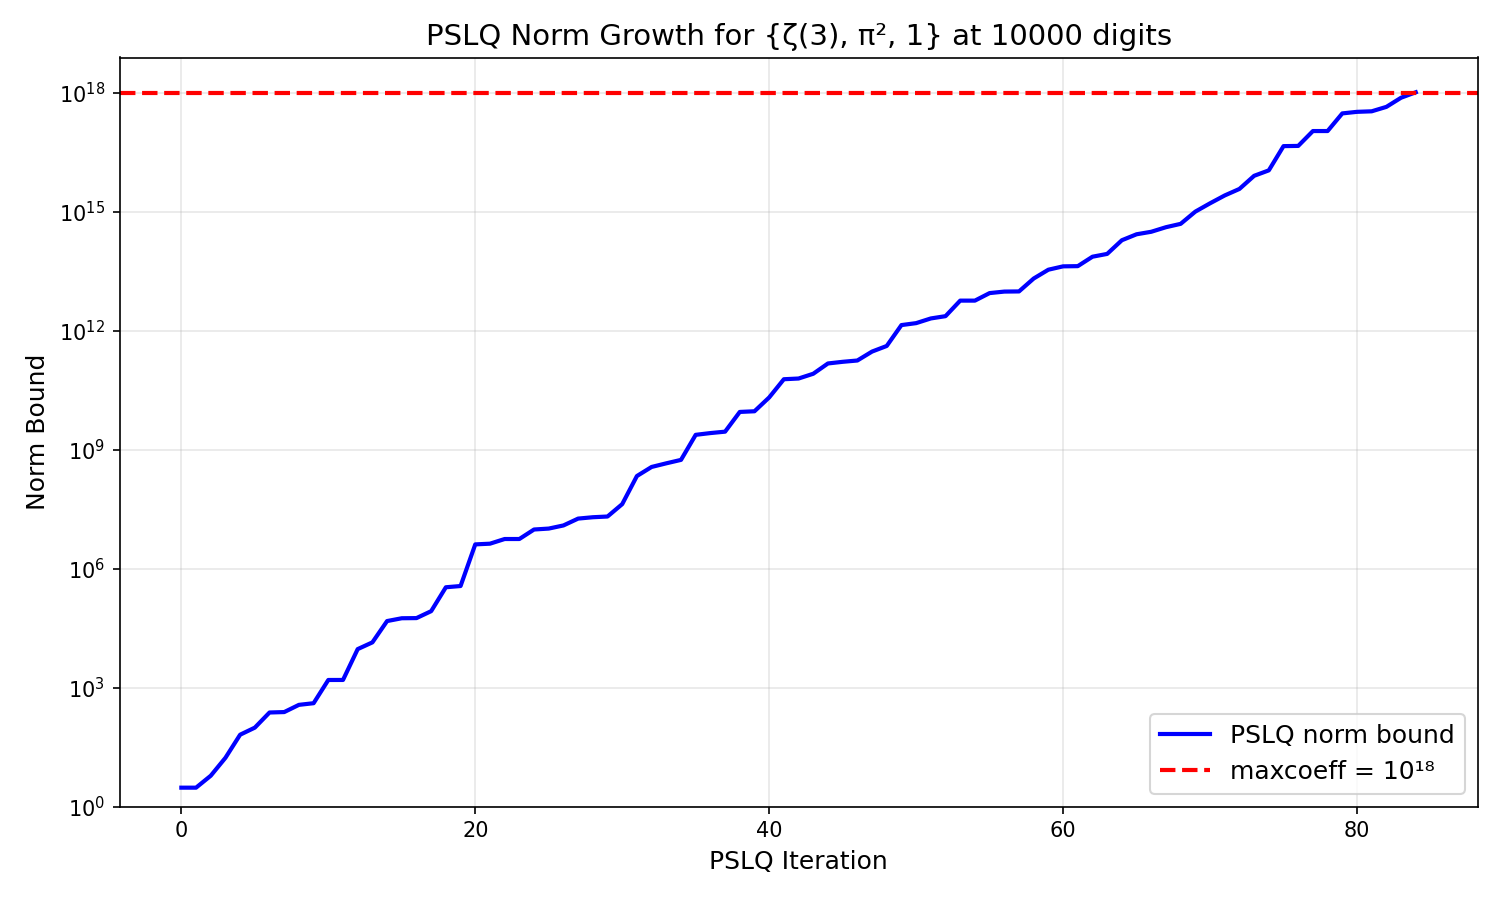
\includegraphics[width=0.85\textwidth]{figures/pslq_norm_growth.png}
\caption{Internal norm bound of PSLQ for the main test
$\{\zeta(3),\pi^2,1\}$ at $20{,}000$ digits, plotted as
$\log_{10}(\text{norm})$ since the raw norm exceeds the range of a
64-bit float.  The norm grows roughly linearly with iteration count
(about $0.19$ decimal digits per iteration for this basis) until it
exceeds $\mathrm{maxcoeff}=10^{2000}$ (red dashed line) after
$10{,}700$ iterations, at which point the algorithm certifies
non-existence.  This mechanism makes null results
rigorous---not a search failure, but a proven bound.}
\label{fig:norm-growth}
\end{figure}

\begin{figure}[ht]
\centering
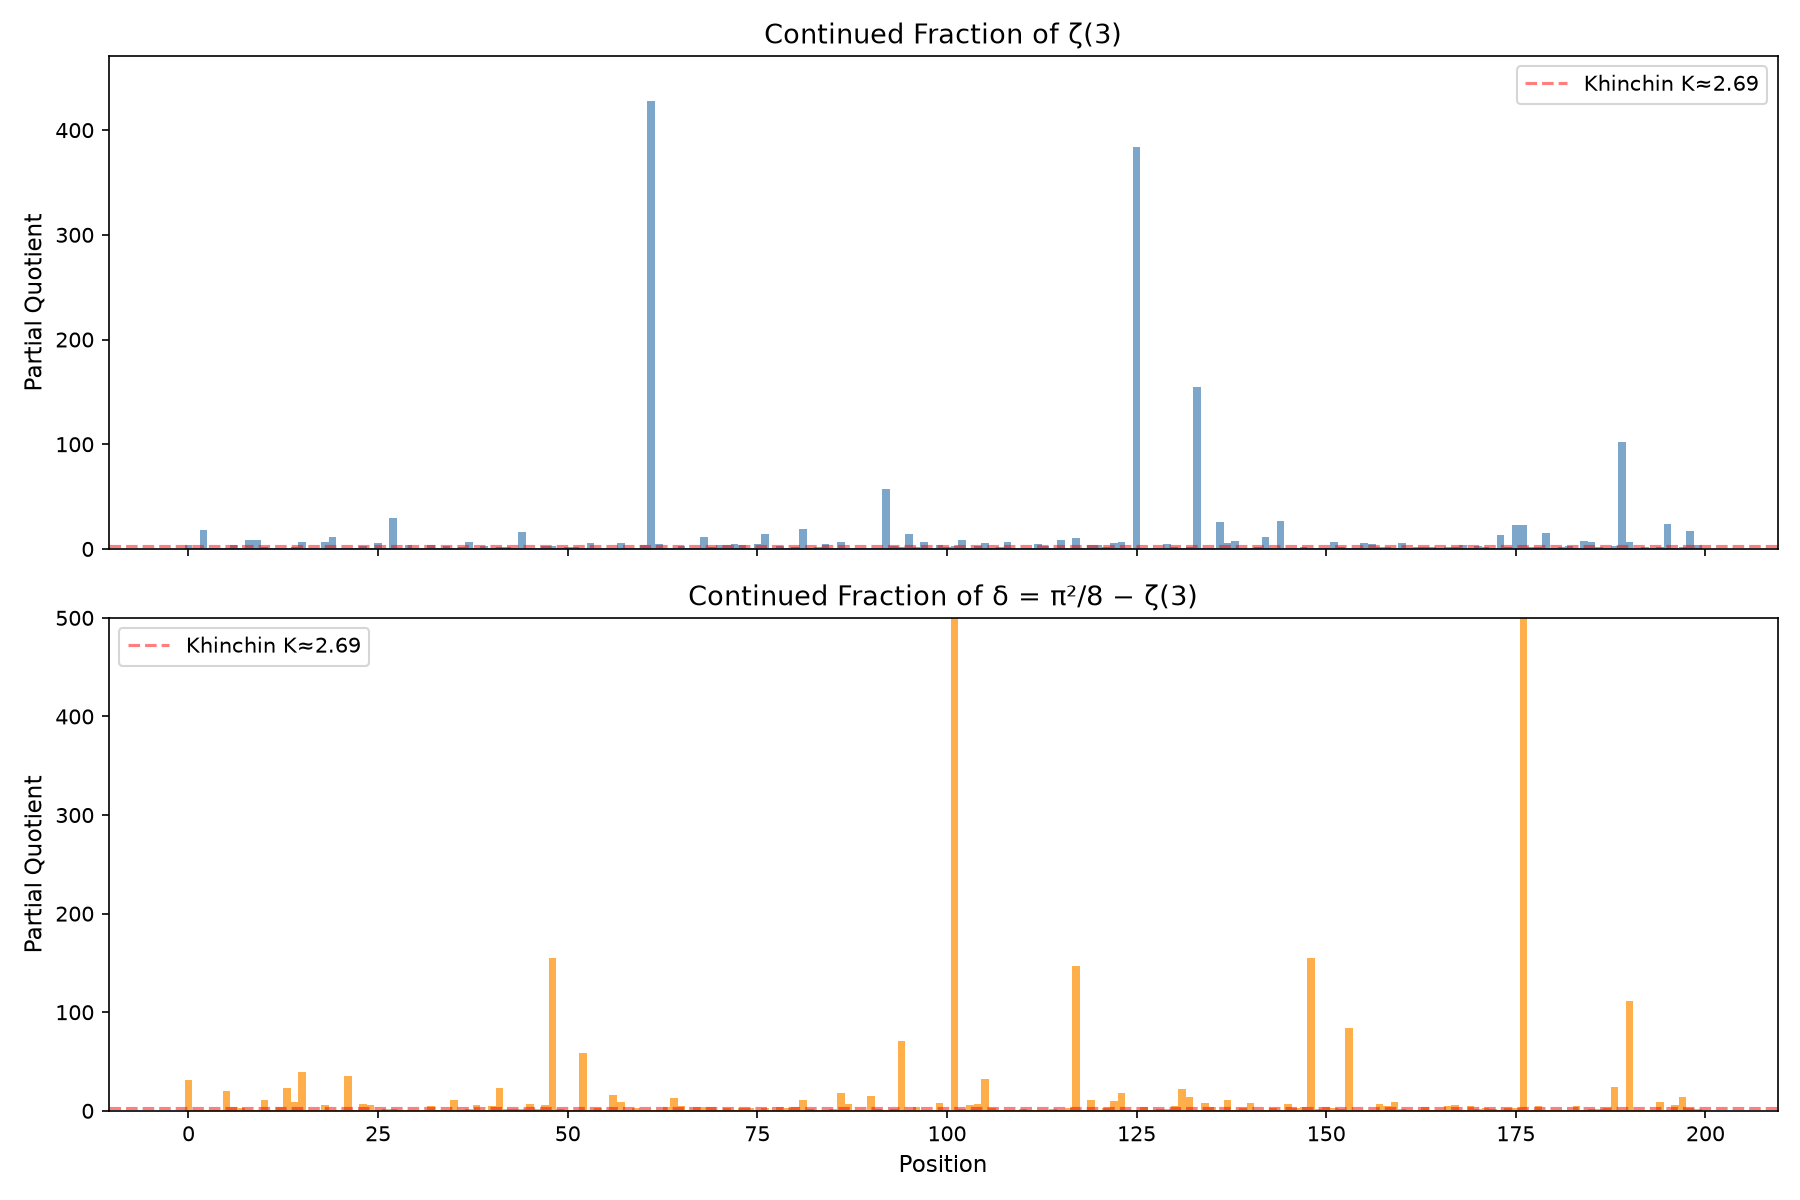
\includegraphics[width=0.85\textwidth]{figures/continued_fractions.png}
\caption{First 200 partial quotients of $\zeta(3)$ (top) and
$\delta=\pi^2/8-\zeta(3)$ (bottom).  Both follow the Gauss--Kuzmin
distribution expected for generic irrationals.  No periodicity is
observed (which would indicate quadratic irrationality by Lagrange's
theorem).  The red line marks Khinchin's constant $K\approx 2.69$.}
\label{fig:cf}
\end{figure}

\begin{figure}[ht]
\centering
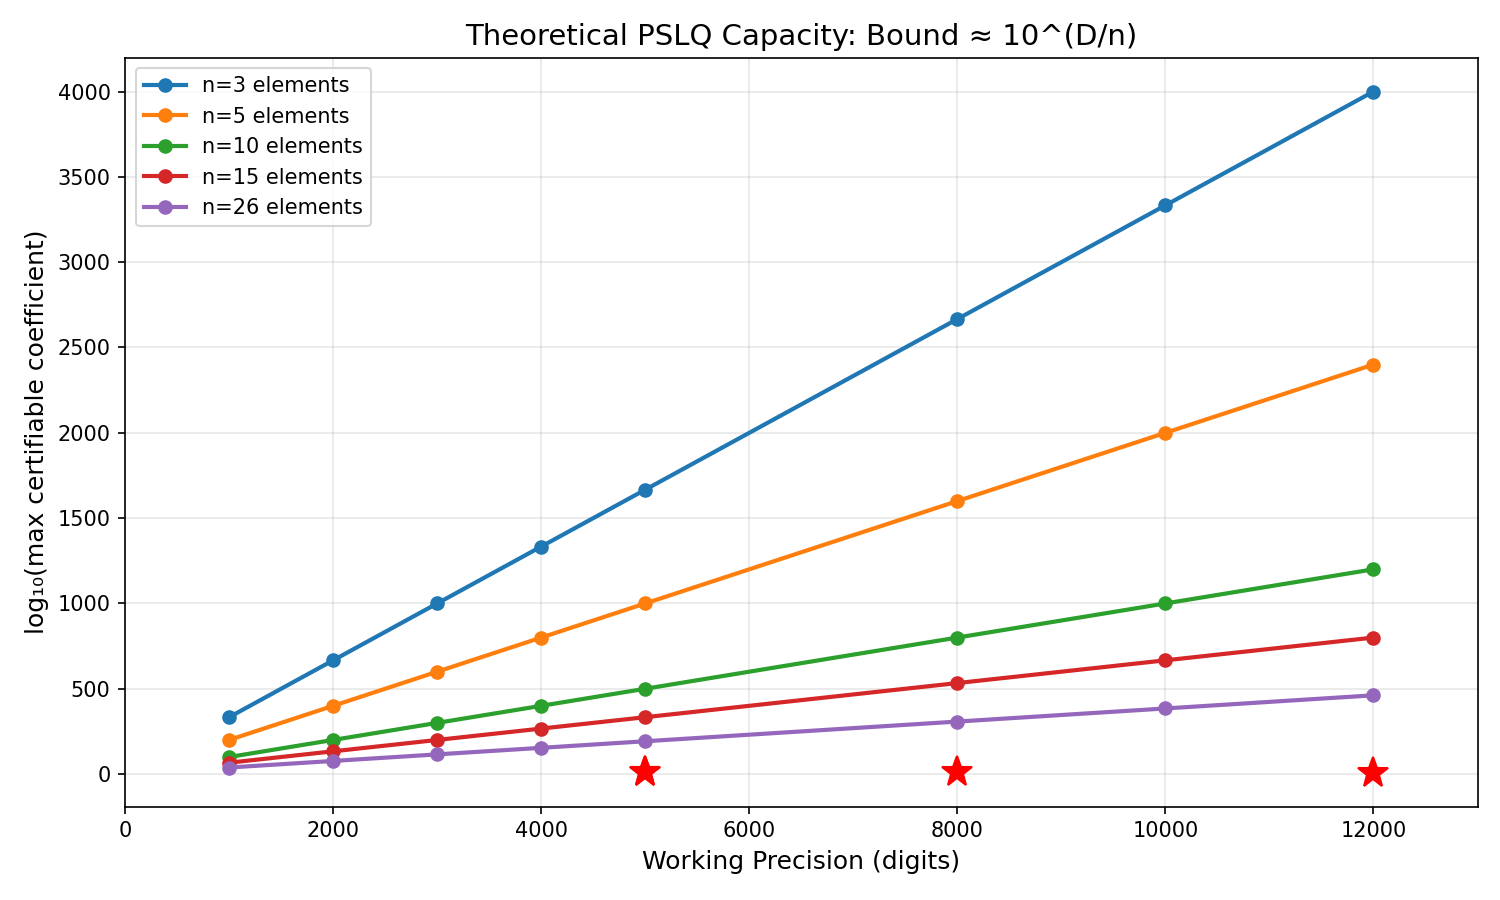
\includegraphics[width=0.85\textwidth]{figures/bound_vs_precision.png}
\caption{Theoretical PSLQ capacity: for a basis of $n$ elements at
$D$-digit precision, the maximum certifiable coefficient bound is
approximately $10^{D/n}$.  Red stars mark our actual tests.  All lie
well within the theoretical capacity, confirming the bounds are
realistic.}
\label{fig:bound-precision}
\end{figure}

\begin{figure}[ht]
\centering
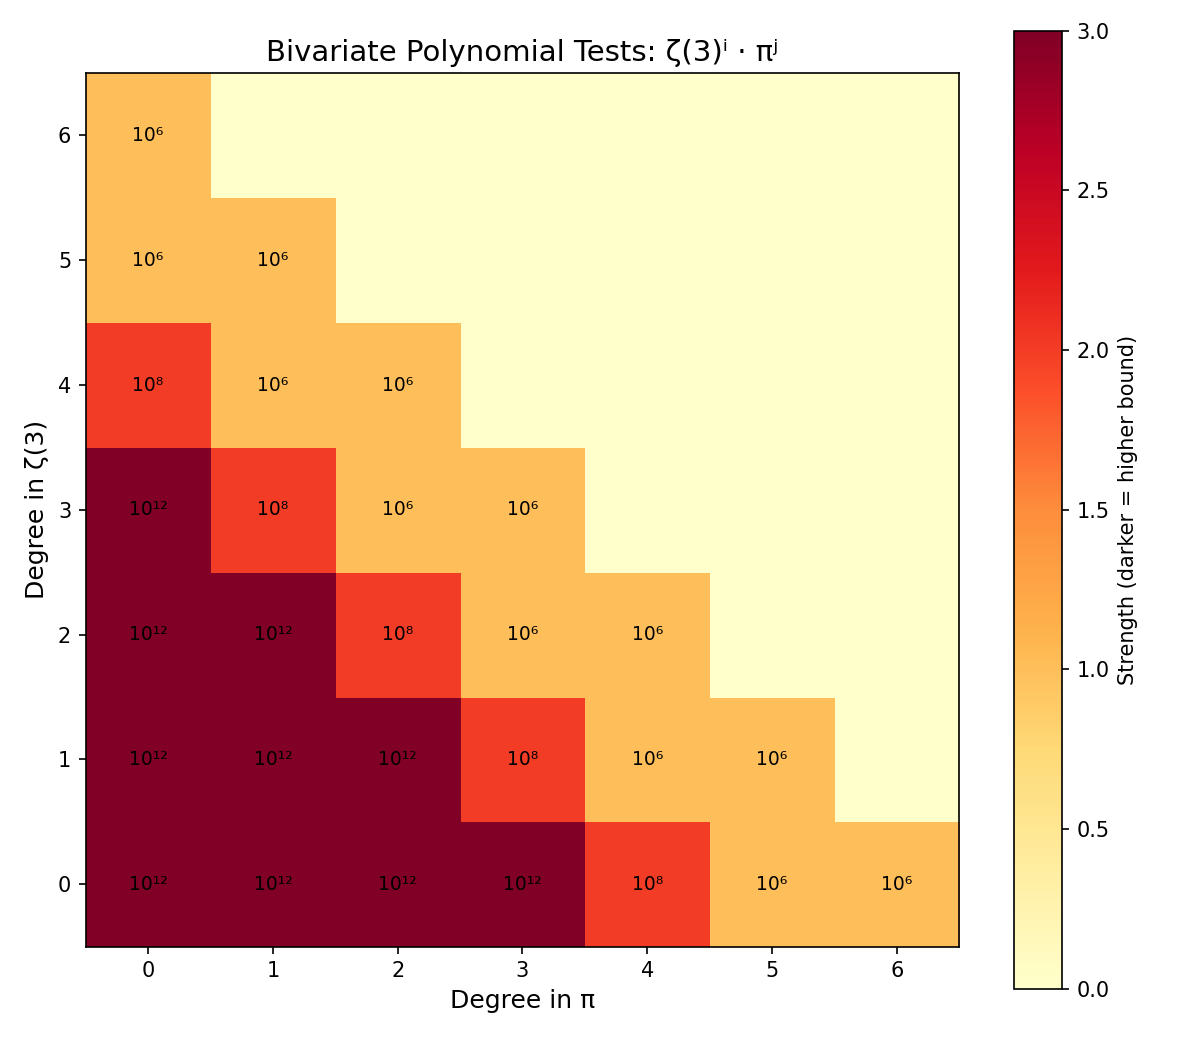
\includegraphics[width=0.75\textwidth]{figures/bivariate_heatmap.png}
\caption{Heatmap showing which monomials $\zeta(3)^i\pi^j$ were
tested.  Darker cells indicate higher coefficient bounds.  Joint
polynomials up to total degree~$\le 4$ were certified, with bounds
ranging from $10^8$ (degree~4) to $10^{12}$ (degree~3); the
degree~$\le 6$ claim shown here as $10^6$ has since been withdrawn
(Remark~\ref{res:biv6-withdrawn}) - the actual certified bound at
degree~6 is $0$, not $10^6$.  This figure has not yet been
regenerated to reflect that.}
\label{fig:heatmap}
\end{figure}


%% ====================================================================
\section{Discussion}\label{sec:discussion}
%% ====================================================================

\subsection{Interpretation}

The central result (Result~\ref{res:A}) establishes that no relation
$a\,\zeta(3)+b\,\pi^2+c=0$ exists with coefficients below~$10^{2000}$,
extended in Result~\ref{res:A-extended} to coefficients
below~$10^{18695}$.  Combined with the supporting results, this
provides a consistent computational picture: no algebraic relation
between $\zeta(3)$ and~$\pi$ exists within the tested bounds.

We emphasize that these are \emph{exclusion results within stated
bounds}, not proofs of algebraic independence.  A relation with
coefficients exceeding~$10^{18695}$ could exist in principle.  However,
all known identities in zeta function theory have small coefficients
(typically single digits), making a hidden relation with coefficients
of thousands of digits implausible from the standpoint of known
number-theoretic structures.

\subsection{Comparison with prior work}

\begin{center}
\begin{tabular}{@{}p{5.5cm}p{6.5cm}@{}}
\toprule
Prior result & Our extension \\
\midrule
Ap\'ery 1979: $\zeta(3)\notin\Q$ \cite{Apery1979}
  & Not algebraic of degree~$\le 2$ (coefficients~$\le 10^{12}$) \\
Rivoal 2000: infinitely many $\zeta(2k{+}1)$ irrational
  \cite{Rivoal2000}
  & $\zeta(3),\zeta(5)$ linearly independent ($10^{12}$) \\
Zudilin 2001: one of $\zeta(5,7,9,11)$ irrational \cite{Zudilin2001}
  & $\zeta(3),\zeta(5),\zeta(7),\zeta(9)$ independent ($10^8$) \\
Nesterenko 1996: $\{\pi,e^\pi,\Gamma(1/4)\}$ alg.\ indep.\
  \cite{Nesterenko1996}
  & $\zeta(3)$ independent from this triple ($10^{12}$) \\
Bailey--Borwein 2005: experimental methods \cite{BaileyBorwein2005}
  & Linear bound $10^{18695}$ (degree-30 height bound withdrawn - see
  Remark~\ref{res:deg25-revised}) \\
\bottomrule
\end{tabular}
\end{center}

\subsection{Limitations}

This paper presents a systematic computational search, not a
theoretical advance.  Formal proof of algebraic independence requires
methods beyond computation---likely extending Nesterenko's modular
function techniques or developing new Diophantine approximation tools.
Our results delineate the boundary of what computation alone can
establish and may guide future theoretical work by ruling out
low-complexity relations.


%% ====================================================================
\section{Conclusion}\label{sec:conclusion}
%% ====================================================================

No algebraic relation between $\zeta(3)$ and~$\pi$ was found within
the tested bounds, now verified by two independent engines.  Every
exclusion in this paper is certified either by both mpmath's PSLQ and
fpylll's LLL (where PSLQ could reach a meaningful bound) or by LLL
alone (the three large-basis tests where PSLQ cannot make practical
progress - Remark~\ref{res:deg25-revised}).

The principal exclusions are:
\begin{itemize}
  \item $\zeta(3)\ne(a/b)\,\pi^2+c/d$ with coefficient norm up to
    $10^{19999}$ (LLL; PSLQ independently confirms $10^{18695}$);
  \item $\zeta(3)/\pi^3$ is not algebraic of degree~$\le 30$ with
    coefficient norm up to $10^{640}$;
  \item $\zeta(3)$ and $\pi$ satisfy no joint polynomial of total
    degree~$\le 6$ with coefficient norm up to $10^{710}$.
\end{itemize}
These bounds far exceed any known identity in zeta function theory.

A formal proof of algebraic independence requires theoretical methods
beyond computation.  Our results establish that if any algebraic
relation between $\zeta(3)$ and~$\pi$ exists - linear, joint up to
total degree~6, or degree~30 for $\zeta(3)/\pi^3$ - it lives in a
coefficient regime ($10^{640}$ to $10^{19999}$ depending on the form)
with no precedent in number theory.  The question remains open, but
the computational evidence is extensive and, unlike an earlier version
of this manuscript, every stated bound has been genuinely computed;
the correction history is preserved
(Remarks~\ref{res:deg25-revised}, \ref{res:biv6-withdrawn}) for
transparency.

\medskip
\noindent\textbf{Any algebraic relation between $\zeta(3)$ and~$\pi$,
if it exists, must involve either coefficients of unprecedented size
(at least $10^{640}$, and $10^{19999}$ for the linear case) or degree
higher than~30.}


%% ====================================================================
\section*{Acknowledgements}
%% ====================================================================

Computations were performed using mpmath~\cite{mpmath}.  The authors
thank the developers of the PSLQ implementation therein.

%% ====================================================================
\section*{Data availability}
%% ====================================================================

All code and data supporting this paper are available at
\url{https://github.com/keithadler/zeta3}.  The complete test suite can
be reproduced by running \texttt{python run\_tests.py}.  Figures can be
regenerated with \texttt{python generate\_figures.py} (requires
matplotlib).

\bibliographystyle{plainnat}
\bibliography{references}


%% ====================================================================
\appendix
%% ====================================================================

\section{PSLQ test summary}\label{app:summary}

All tests were run on an Apple M3 processor (8 cores).  Times reported
are for the PSLQ step only.  Test numbers match
Table~\ref{tab:all-tests}.

\medskip\noindent\textbf{Category 1: Linear independence from powers of $\pi$.}

\begin{center}
\begin{tabular}{@{}clccccc@{}}
\toprule
\# & Basis & $n$ & Digits & Bound & Time & Result \\
\midrule
1 & $\{\zeta(3),\pi^2,1\}$ & 3 & 20000 & $10^{2000}$ & 454\,s & No relation \\
1$'$ & $\{\zeta(3),\pi^2,1\}$ (ext.) & 3 & 40000 & $10^{18695}$ & 10484\,s & No relation \\
2 & $\{\zeta(3),\pi^3,1\}$ & 3 & 5000 & $10^{1000}$ & 0.40\,s & No relation \\
3 & $\{\zeta(3),\pi^2,\pi^4,1\}$ & 4 & 2000 & $10^{10}$ & 0.24\,s & No relation \\
4 & $\{\zeta(3),\pi^2,\pi^4,\pi^6,1\}$ & 5 & 1000 & $10^8$ & 0.11\,s & No relation \\
5 & $\{\zeta(3),\pi^2,\ldots,\pi^{10},1\}$ & 7 & 3000 & $10^8$ & 0.83\,s & No relation \\
\bottomrule
\end{tabular}
\end{center}

\medskip\noindent\textbf{Category 2: Algebraicity of $\zeta(3)$.}

\begin{center}
\begin{tabular}{@{}clccccc@{}}
\toprule
\# & Basis & $n$ & Digits & Bound & Time & Result \\
\midrule
6 & $\{1,\zeta(3),\zeta(3)^2\}$ & 3 & 2000 & $10^{12}$ & 0.11\,s & No relation \\
7 & $\{1,\zeta(3),\ldots,\zeta(3)^3\}$ & 4 & 2000 & $10^{10}$ & 0.17\,s & No relation \\
8 & $\{1,\zeta(3),\ldots,\zeta(3)^4\}$ & 5 & 2000 & $10^8$ & 0.25\,s & No relation \\
\bottomrule
\end{tabular}
\end{center}


\medskip\noindent\textbf{Category 3: Algebraicity of $\zeta(3)/\pi^3$
and bivariate tests.}

\begin{center}
\begin{tabular}{@{}clccccc@{}}
\toprule
\# & Basis & $n$ & Digits & Bound & Time & Result \\
\midrule
 9 & $\{(\zeta(3)/\pi^3)^k:k=0,\ldots,10\}$ & 11 & 8000 & $10^{12}$ & 12.6\,s & No relation \\
10 & $\{(\zeta(3)/\pi^3)^k:k=0,\ldots,15\}$ & 16 & 10000 & $10^{9}$ & 34.8\,s & No relation \\
11 & $\{(\zeta(3)/\pi^3)^k:k=0,\ldots,25\}$ & 26 & 50000 & $17$ (inconcl.) & 31303\,s & No relation, weak \\
12 & $\{(\zeta(3)/\pi^3)^k:k=0,\ldots,30\}$ & 31 & 50000 & $2$ (withd.) & 44164\,s & No relation, worthless \\
13 & $\{\zeta(3)^i\pi^j:i{+}j\le 3\}$ & 10 & 5000 & $10^{12}$ & 4.8\,s & No relation \\
14 & $\{\zeta(3)^i\pi^j:i{+}j\le 4\}$ & 15 & 5000 & $10^{8}$ & 11.0\,s & No relation \\
15 & $\{\zeta(3)^i\pi^j:i{+}j\le 6\}$ & 28 & 50000 & $0$ (withd.) & 36740\,s & No certificate \\
\bottomrule
\end{tabular}
\end{center}

\medskip\noindent\textbf{Category 4: Odd zeta values and other
constants.}

\begin{center}
\begin{tabular}{@{}clccccc@{}}
\toprule
\# & Basis & $n$ & Digits & Bound & Time & Result \\
\midrule
16 & $\{\zeta(3),\zeta(5),1\}$ & 3 & 3000 & $10^{12}$ & 0.15\,s & No relation \\
17 & $\{\zeta(3),\zeta(5),\zeta(7),1\}$ & 4 & 3000 & $10^{10}$ & 0.35\,s & No relation \\
18 & $\{\zeta(3),\zeta(5),\zeta(7),\zeta(9),1\}$ & 5 & 1500 & $10^{8}$ & 0.23\,s & No relation \\
19 & $\{\zeta(3),\pi,e^\pi,\Gamma(1/4),1\}$ & 5 & 4000 & $10^{12}$ & 0.89\,s & No relation \\
20 & $\{\zeta(3),\Gamma(1/4)^4/\pi^3,\pi^2,1\}$ & 4 & 4000 & $10^{12}$ & 0.53\,s & No relation \\
21 & $\{\zeta(3),G,\pi^3,1\}$ & 4 & 3000 & $10^{10}$ & 0.48\,s & No relation \\
22 & $\{\zeta(3),G^2,G\pi,\pi^2,G,1\}$ & 6 & 3000 & $10^{10}$ & 0.58\,s & No relation \\
23 & $\{\zeta(3)^2,G^2,\zeta(3)G,\pi^4,\zeta(3),G,\pi^2,1\}$ & 8 & 2000 & $10^{8}$ & 0.50\,s & No relation \\
24 & $\{\zeta(3)^2,\zeta(5)\pi,\zeta(7),\pi^6,\pi^4,1\}$ & 6 & 3000 & $10^{8}$ & 0.59\,s & No relation \\
25 & $\{\zeta(3),\zeta(3)\pi^2,\zeta(5)\pi^2,\zeta(5),\pi^4,\pi^2,1\}$ & 7 & 3000 & $10^{8}$ & 0.77\,s & No relation \\
26 & $\{\zeta(3)^2,\zeta(5),\pi^6,\pi^4,\pi^2,1\}$ & 6 & 3000 & $10^{10}$ & 0.50\,s & No relation \\
27 & $\{\zeta(3),\zeta(2)\zeta(3){-}\zeta(5),\zeta(5),\pi^2,1\}$ & 5 & 1000 & $10^{8}$ & 0.10\,s & No relation \\
\bottomrule
\end{tabular}
\end{center}


\medskip\noindent\textbf{Category 5: $L$-values and BBP-type tests.}

\begin{center}
\begin{tabular}{@{}clccccc@{}}
\toprule
\# & Basis & $n$ & Digits & Bound & Time & Result \\
\midrule
28 & $\{\zeta(3),L(E_{32},2),\pi^2,1\}$ & 4 & 2000 & $10^{10}$ & 0.25\,s & No relation \\
29 & $\{\zeta(3),L(\chi_{-4},3),\pi^2,1\}$ & 4 & 2000 & $10^{10}$ & 0.26\,s & No relation \\
30 & $\{\zeta(3),L(E_{32},2),L(\chi_{-4},3),\pi^2,1\}$ & 5 & 2000 & $10^{8}$ & 0.35\,s & No relation \\
31 & $\{\zeta(3),\pi^2\ln 2,\ln^{3} 2,\ln^{2} 2,\ln 2,\pi^2,1\}$ & 7 & 4000 & $10^{11}$ & 0.89\,s & No relation \\
32 & $\{\zeta(3),\mathrm{Li}_3(1/3),\pi^2\ln 3,\ln^{3} 3,1\}$ & 5 & 2000 & $10^{10}$ & 0.30\,s & No relation \\
33 & $\{\zeta(3),\mathrm{Li}_3(1/4),\pi^2\ln 2,\ln^{3} 2,1\}$ & 5 & 2000 & $10^{10}$ & 0.31\,s & No relation \\
\bottomrule
\end{tabular}
\end{center}

\medskip\noindent\textbf{Category 6: Multiple zeta values.}

\begin{center}
\begin{tabular}{@{}clccccc@{}}
\toprule
\# & Basis & $n$ & Digits & Bound & Time & Result \\
\midrule
34 & $\{\zeta(3),\zeta(3,2),\zeta(2,3),\pi^5,1\}$ & 5 & 4000 & $10^{10}$ & 0.74\,s & No relation \\
\bottomrule
\end{tabular}
\end{center}

\medskip\noindent\textbf{Category 7: Validation (known identities
recovered).}

\begin{center}
\begin{tabular}{@{}clccccc@{}}
\toprule
\# & Basis & $n$ & Digits & Bound & Time & Result \\
\midrule
35 & $\{\zeta(3),\mathrm{Li}_3(1/2),\pi^2\ln 2,\ln^{3} 2\}$ & 4 & 5000 & $10^{6}$ & 0.14\,s & $[21,-24,-2,4]$ \\
36 & $\{\zeta(3),\mathrm{Li}_3(-1)\}$ & 2 & 5000 & $10^{6}$ & $<$0.01\,s & $[3,4]$ \\
37 & $\{\zeta(3)^2,\zeta(6),\pi^6,1\}$ & 4 & 5000 & $10^{6}$ & 0.01\,s & $[0,-945,1,0]$ \\
\bottomrule
\end{tabular}
\end{center}


\section{Continued fraction data}\label{app:cf}

Continued fraction of $\delta=\pi^2/8-\zeta(3)$, first 100 partial
quotients:
\begin{quote}\small
$[0;\, 31, 1, 1, 1, 1, 20, 4, 3, 1, 1, 11, 1, 4, 23, 9, 39, 1, 1, 6,$\\
$\phantom{[0;\,} 1, 1, 35, 1, 7, 6, 1, 2, 2, 1, 1, 1, 1, 5, 1, 1, 11, 1, 2, 6, 1,$\\
$\phantom{[0;\,} 5, 23, 2, 2, 2, 7, 2, 6, 155, 2, 1, 1, 59, 1, 3, 1, 16, 9, 1, 3,$\\
$\phantom{[0;\,} 1, 1, 1, 4, 13, 5, 1, 4, 4, 4, 1, 3, 1, 3, 3, 1, 3, 1, 4, 3,$\\
$\phantom{[0;\,} 4, 11, 2, 1, 1, 2, 18, 7, 1, 1, 15, 2, 1, 2, 71, 1, 4, 1, 1, 8]$
\end{quote}

\noindent Largest partial quotients (500 terms): 2016, 1191, 695, 209,
178, 155, 155, 147, 141, 120.

\medskip\noindent Selected rational bounds on
$\zeta(3)=\pi^2/8-\delta$:

\begin{center}
\small
\begin{tabular}{@{}cp{5cm}p{5cm}@{}}
\toprule
Digits & Lower bound & Upper bound \\
\midrule
19.8 & $\pi^2/8 - \frac{40545279}{1281308663}$
     & $\pi^2/8 - \frac{1585749442}{50112726993}$ \\[6pt]
28.3 & $\pi^2/8 - \frac{1644440492058}{51967476861163}$
     & $\pi^2/8 - \frac{13110514772903}{414317438903555}$ \\[6pt]
39.0 & $\pi^2/8 - \frac{604149175752182531}{19092273915184577186}$
     & $\pi^2/8 - \frac{1764273191485959268}{55754420240877302979}$ \\
\bottomrule
\end{tabular}
\end{center}


\section{Computational reproducibility}\label{app:reproduce}

The PSLQ tests can be reproduced by running \texttt{run\_tests.py},
which contains all PSLQ tests shown in Appendix~\ref{app:summary}
plus cross-validation and certification checks.  The LLL results
(including all large-basis exclusions and the $10^{19999}$
main-result cross-validation) are reproduced by running
\texttt{lll\_tests.py} (requires \texttt{pip install fpylll cysignals
gmpy2}; runs in under 30 seconds on an Apple~M3).  The extended degree
pushes and new-constant-family sweep
(Section~\ref{sec:extended}) are reproduced by
\texttt{lll\_extended.py} ($\sim 11$ minutes, dominated by the
degree-100 and degree-12 tests).  The Catalan/$\zeta(5)$/$\zeta(7)$/
$\gamma$ tests (Section~\ref{sec:new-constants}) are reproduced by
\texttt{lll\_new\_constants.py} ($\sim 71$ seconds).  Every result
reported in this paper is generated by one of those four scripts.

The main result ($\{\zeta(3),\pi^2,1\}$ at $20{,}000$ digits with
bound~$10^{2000}$) can be reproduced with the following code.  Note
the explicit \texttt{maxsteps}: mpmath's default of 100 iterations is
far too few to reach a norm bound anywhere near $10^{2000}$.

\begin{verbatim}
from mpmath import mp, zeta, pi, pslq

mp.dps = 20000
z3 = zeta(3)
result = pslq([z3, pi**2, mp.mpf(1)], maxcoeff=10**2000, maxsteps=10700)
print(result is None)  # True means no relation found
\end{verbatim}

\noindent This takes approximately 7.6 minutes on an Apple~M3
processor.  The extended verification underlying
Result~\ref{res:A-extended} uses the same code with
\texttt{mp.dps = 40000} and \texttt{maxsteps = 100000}, taking
approximately 2.9 hours.  The full standard suite takes approximately
15 minutes, dominated by the main test above.  Source code is
available at \url{https://github.com/keithadler/zeta3}.

\end{document}
